\section{The \grackle{} Chemistry and Cooling Library}

The \grackle{} project
\citep[][\url{https://grackle.readthedocs.io}]{2017MNRAS.466.2217S} is
an open-source library for computing the chemistry and radiative
cooling in astrophysical simulations and models.  The
\grackle{} library exposes functions necessary for computing the
thermal and chemical evolution of a collection of fluid elements carried by a
simulation.  These fluid elements can be either Eulerian (cells),
Lagrangian (particles), or a hybrid (e.g., moving mesh) with
application programming interfaces (APIs)
existing for codes written in C, C++, Fortran, and Python.  The
physical processes covered by the solver make it applicable to a broad
range of astrophysical topics.  Among
other metrics, the utility of \grackle{} can be demonstrated in two
important ways.  First, \grackle{} is a key component of the AGORA
\citep{2014ApJS..210...14K, 2016ApJ...833..202K} simulation comparison
project.  Comparing nine different simulation codes over multiple
galaxy formation problems, the AGORA project is the first
undertaking to include such a large fraction of the galaxy formation research
community.
%% An example of this cross-platform comparison enabled by
%% \grackle{} is shown in Figure \ref{fig:AGORA}.
Second, \grackle{} has
seen widespread adoption and use outside of participation in AGORA.
In total, \grackle{} has been adopted by at least 14 different
simulation codes:
AREPO, ART-I, ART-II, ChaNGa, Cosmos++, Enzo, Gadget, GAMER, GASOLINE, Gear,
Gizmo, RAMSES, SPHS, and SWIFT
\citep{2010MNRAS.401..791S, 1999PhDT........25K, 2002ApJ...571..563K,
2008ApJ...672...19R, 2004NewA....9..137W, 2006MNRAS.373.1074S,
2003ApJS..147..177A, 2005ApJ...635..723A, 2014ApJS..211...19B,
2005MNRAS.364.1105S, 2010ApJS..186..457S, 2004NewA....9..137W,
2012A&A...538A..82R, 2012ASPC..453..141R, 2015MNRAS.450...53H,
2002A&A...385..337T, 2012MNRAS.422.3037R, 2013arXiv1309.3783G,
2016arXiv160602738S}.

%% \begin{figure}[h]
%% \begin{center}
%% 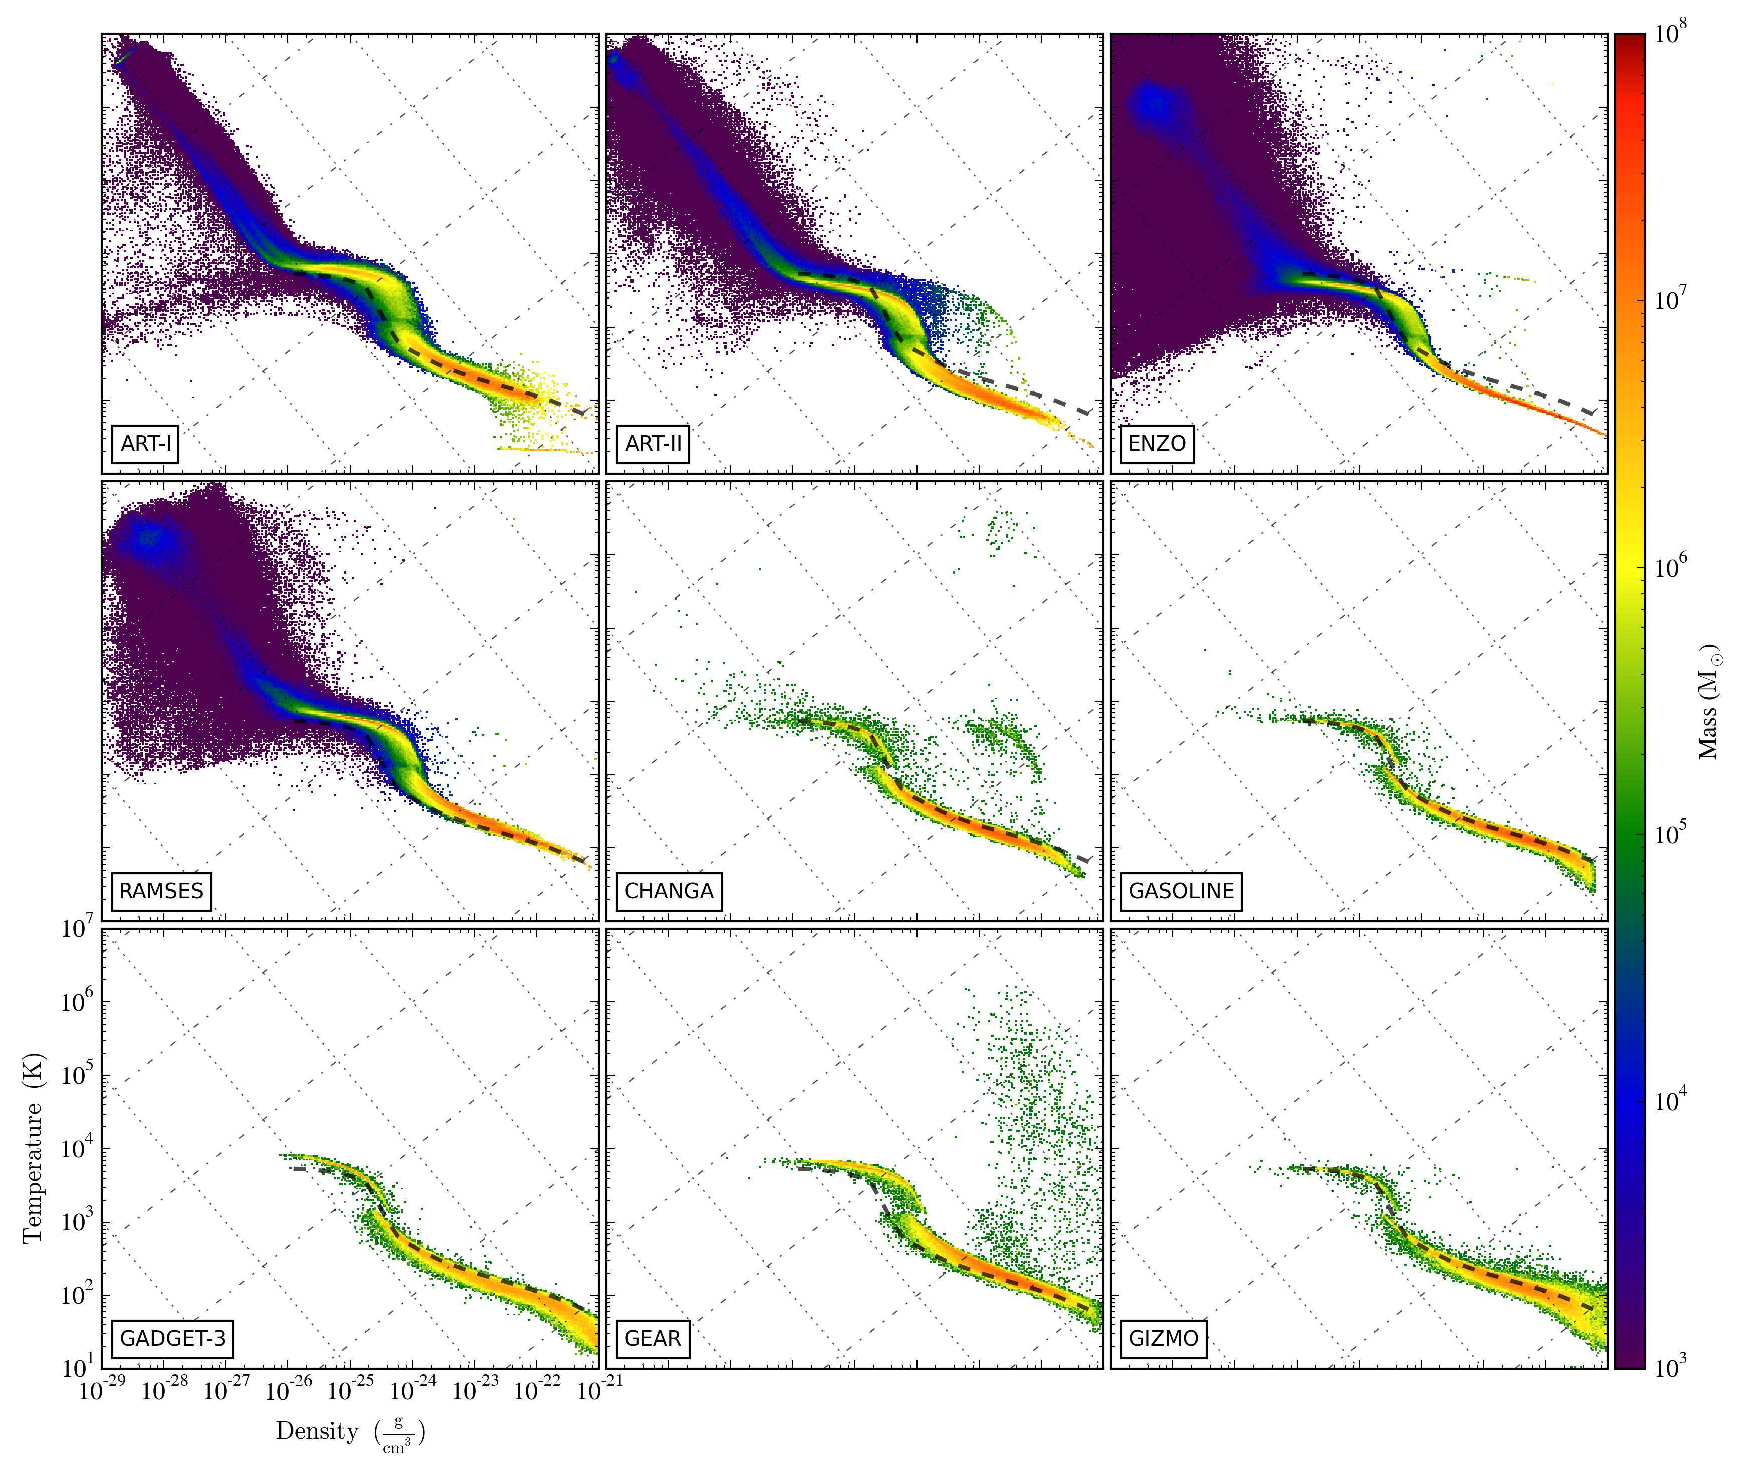
\includegraphics[width=0.92\textwidth]{figures/fig17.eps}
%% \caption{A comparison of nine simulation codes in the AGORA project, all using
%%   \grackle{}.  The panels show the probability distribution function
%%   in bins of density and temperature for the gas in isolated galaxy
%%   simulations.  Each simulation used an identical idealized setup,
%%   prescriptions for star formation and feedback, and radiative cooling
%%   provided by the \grackle{} library
%%   \citep[from][]{2016ApJ...833..202K}.}
%% \label{fig:AGORA}
%% \end{center}
%% \vspace*{-2\baselineskip}
%% \end{figure}

\noindent
{\bf As an open-source project, \grackle{} plays two major roles:}
\begin{enumerate}
\item It provides access via a universal API to necessary functionality
that can be difficult for individual research groups to develop or
maintain on their own.  This increases overall productivity and
enables comparison and collaboration.
\item By actively encouraging contribution though personal engagement
and open-source software best practices, the widely adopted API serves
as a conduit for dissemination of new methods and research results to
the community.
\end{enumerate}
However, for \grackle{} to continue to be a useful resource, we must
ensure that the code is more inviting to new contributors, does not
become a performance bottleneck on next-generation computing facilities, 
and is flexible enough to be adapted to new areas of research.
The purpose of this proposal is to support a
series of development tasks necessary to keep up with the demands of
current users, broaden
applicability, and to make \grackle{} a
self-sustaining community project by the grant period's end.  While
\grackle{} is developed completely openly, and
is thus in a continuous state of development release, the proposed
tasks and their order of completion have been designed to yield
regular major stable releases at the end of each year.
%% The proposed tasks and their order of
%% completion have been designed to incrementally make the code more
%% attractive to external contribution and adoption by a wider audience.
%% The completion of each task will be marked by a major release of the
%% code.

\subsection{\grackle{} API}\label{sec:arch}

\grackle{} is a full-featured solver for gas chemistry and radiative
cooling with an API that is designed to minimize backward
compatibility issues and is straightforward to implement in simulation
codes written in C, C++, Fortran, and Python.  All functionality is
parallelized with OpenMP and can be used in hybrid MPI/OpenMP
frameworks.
%% The Python interface includes additional features to aid
%% in semi-analytical modeling and debugging.

\grackle{} provides a non-equilibrium (NEQ) primordial chemistry solver for
atomic and molecular species of H, D, and He, including H$_{2}$
formation via three-body reactions \citep{2002Sci...295...93A,
2011ApJ...726...55T} and on dust-grain surfaces
\citep{1979ApJS...41..555H, 2000ApJ...534..809O, 2014ApJ...783...75M},
H$_{2}$ formation 
heating \citep{2009Sci...325..601T}, collision-induced H$_{2}$
emission \citep{2004MNRAS.348.1019R}, and HI
\citep{2013MNRAS.430.2427R} and H$_{2}$ \citep{2012MNRAS.425L..51W}
self-shielding.  The cooling from heavy elements up to atomic number
30 (Zn) is calculated by interpolating over tables of cooling and
heating rates created with the photo-ionization software,
\texttt{Cloudy} \citep{2013RMxAA..49..137F}.  These
tables are generated through expensive python scripts and stored in HDF5 files
included with the \grackle{} source.  For
increased speed at the expense of accuracy, the cooling from
primordial elements can also be computed using these tables.  In
addition to tables calculated assuming collisional ionization only
(i.e., no incident radiation), cooling tables have been created for two
different ultraviolet (UV) background models, those of \citet{2009ApJ...703.1416F}
and \citet{2012ApJ...746..125H}, in order to mimic the effects of
reionization.  For radiative transfer codes or simulation codes that
support radiation hydrodynamics, \grackle{} also allows the user to supply
photo-ionization and photo-heating rates for each computational
element.  Arrays of arbitrary specific and volumetric heating
rates may be supplied to account for heating from stellar feedback
models and additional radiation sources.
%% Between these different models and
%% phenomena, nearly the entire collection of relevant radiative processes in
%% astrophysical plasmas are tracked and accounted for in \grackle{}.

The \grackle{} library exposes a series of functions useful to a
hydrodynamic simulation, such as evolving the chemistry network over a
time-step and calculating the instantaneous cooling time.
%% : 1) \texttt{solve\_chemistry} for iterating
%% the chemistry network and updating the species densities and internal
%% energy over a given time-step, and 2)
%% \texttt{calculate\_cooling\_time}, 3) \texttt{calculate\_pressure}, 4)
%% \texttt{calculate\_temperature}, and 5) \texttt{calculate\_gamma} for
%% computing the instantaneous cooling time, thermal pressure,
%% temperature, and ratio of specific heats, respectively.
Most of the
code's behavior is controlled by run-time parameters stored within a C
\texttt{struct} that is accessible from the main \grackle{} header
file.  The solver can be run with varying levels of sophistication,
including fully tabulated cooling, atomic chemistry only (6-species,
H, H$^{+}$, He, He$^{+}$, He$^{++}$, e$^{-}$), and additional tiers of
molecular chemistry (9-species adding H$_{2}$, H$_{2}^{+}$, H$^{-}$
and 12-species adding D, D$^{+}$, and HD).  Each of these requires a
different number of fields to be carried by the simulation code.  This
functionality is exposed through an API that has been designed to
minimize the possibility of future development breaking backward
compatibility.

\grackle{} has been designed to maximize scientific productivity on
high performance computing systems while maintaining an interface that
is immediately useful to people at many different levels of
experience.
All functionality is easily accessible to codes written
in C, C++, and Fortran.  \grackle{} comes with compilable,
runnable examples in each of the above languages demonstrating all
available functions.  A Python module, \texttt{pygrackle},
exposes the main functionality and helper functions useful in
semi-analytic models \citep[e.g.,][]{2016ApJ...820...71C,
  2016MNRAS.459.4209A}, debugging, and education.  Sample
figure-producing scripts are included in the source (see Figure
\ref{fig:freefall}). \texttt{pygrackle's}
dependencies (\texttt{NumPy}, \texttt{Cython}, and \yt{}) are
installable by Python package managers, \texttt{Conda}
and \texttt{pip}.
%\subsection{\texttt{pygrackle}: The Python Interface}
%% \texttt{pygrackle} provides a lower barrier to
%% entry for accessing \grackle{}'s functionality and thus can be
%% useful for semi-analytical models \citep[e.g.,][]{2016ApJ...820...71C,
%% 2016MNRAS.459.4209A}, debugging, and education.  The
%% \texttt{pygrackle} package is distributed with the \grackle{} source
%% and can be installed once the library has been compiled.  The
%% additional Python packages on which \texttt{pygrackle} is built
%% (\texttt{NumPy}, \texttt{Cython}, and \yt{}) are
%% installable by popular Python package managers, like \texttt{Conda}
%% and \texttt{pip}.

%% \texttt{pygrackle} uses an Object-Oriented design centered around
%% \texttt{FluidContainer} objects with the code \grackle{} functions
%% accessible as class methods. The \texttt{FluidContainer} stores field
%% values as \texttt{NumPy} arrays with enhanced functionality, provided
%% by \yt{}, that endows values with symbolically expressable and
%% convertible units.  For example, an array, \texttt{x}, of densities in units of
%% g/cm$^{3}$, can undergo unit conversion by doing:
%% \texttt{x.to("Msun/kpc**3")}.


%% To maintain a single function signature,
%% regardless of chosen settings, field arrays are attached to pointers
%% within a C \texttt{struct} that is passed to the primary functions.
%% With this technique, new features requiring additional fields can be
%% added without altering function signatures, making the code
%% effectively backward compatible indefinitely.  This was an explicit
%% design decision made by the project to minimize future work required
%% by simulation codes using \grackle{}.

\begin{figure}
\centering
\begin{subfigure}{.48\textwidth}
  \centering
  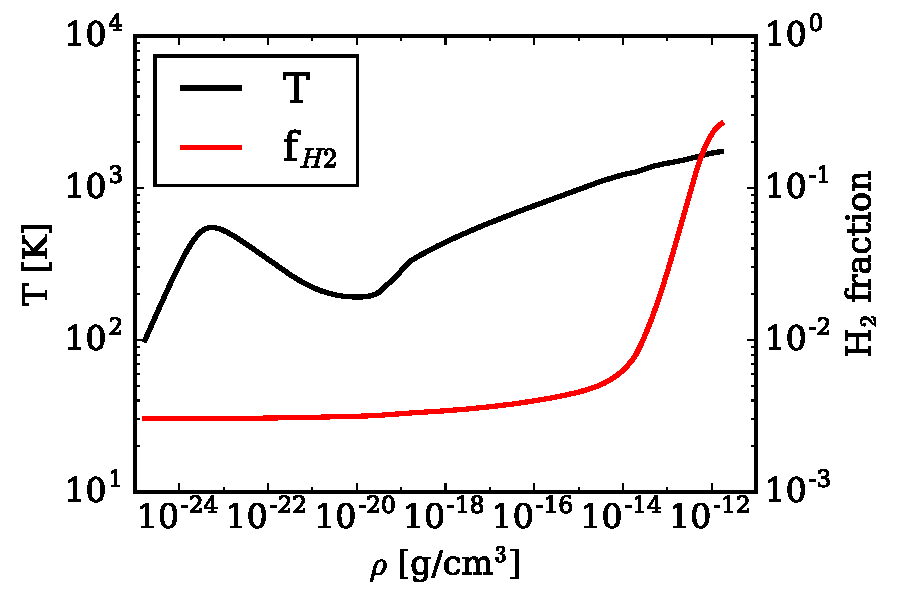
\includegraphics[width=0.98\textwidth]{figures/freefall.pdf}
  \caption{Output from the free-fall collapse\\ model sample script
    using the \texttt{pygrackle}\\Python wrapper.}
  \label{fig:freefall}
\end{subfigure}%
\begin{subfigure}{.42\textwidth}
  \centering
  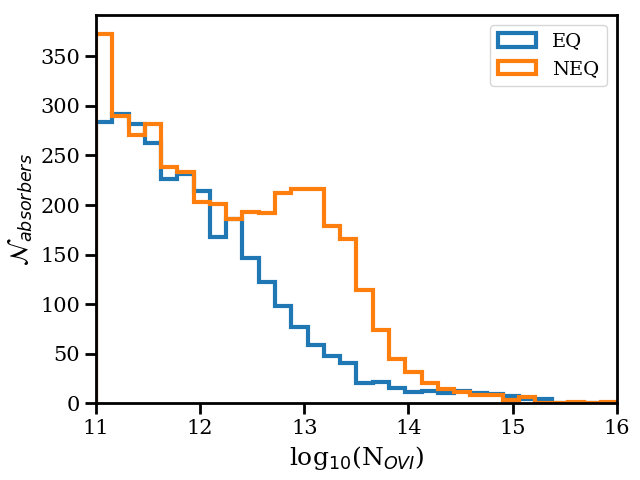
\includegraphics[width=0.98\textwidth]{figures/unmatched_absorbers.png}
  \caption{Number of absorption systems of five times
    ionized O vs. column density for an \enzo{} simulation run
    with equilibrium metal cooling (EQ, \grackle{}) and a NEQ O
    ionization network made by \dengo{} (NEQ).}
  \label{fig:dengo}
\end{subfigure}%
\vspace*{-0.5\baselineskip}
%% \caption{Output from sample \texttt{pygrackle} scripts included in the \grackle{}
%%   source.}
\label{fig:evolve}
\vspace*{-1\baselineskip}
\end{figure}

\grackle{} is built upon widely used packages in the ecosystem of
scientific software.
%% As a library, the aim is to provide
%% functionality to the most commonly used programming languages in
%% scientific computing, namely, C, C++, Fortran, and Python.
The core
library is written in a combination of C and Fortran with the strategy
of using Fortran for the computationally expensive internal machinery
and C for user-facing functions and data storage.  The single
additional dependency is
HDF5\footnote{\url{https://www.hdfgroup.org/HDF5/}}, used for reading
cooling, heating,
and UV background rate data from input files.  HDF5 was chosen because
\grackle{}'s input files contain many data tables and the hierarchical
format makes them easily discoverable without prior knowledge of the
layout, allowing them to be reused for other purposes.  The Python
interface is built upon a number of widely used Python packages, including
\texttt{NumPy}, \texttt{Cython}, and
\yt{}\footnote{\url{http://www.numpy.org/}, \url{http://cython.org/},
  and \url{http://yt-project.org/}, respectively} \citep[][an SI2-funded
project]{2011ApJS..192....9T}.  The project also utilizes:
Mercurial for version control; BitBucket.org for repository hosting;
Sphinx for documentation; readthedocs.org for documentation
hosting; pytest for testing; and BitBucket Pipelines for continuous
integration testing.

\subsection{The Core Library}
\label{sec:core-library}

\noindent
{\bf Methodology}
Chemistry networks are challenging to solve because the time-scales of
reactions involved vary by many orders of magnitude.  These ``stiff''
networks are often solved using implicit methods, as they are able to
take longer time-steps than explicit methods, which are limited by the
shortest time-scale within the network.  However, a number of factors
can make an explicit scheme more attractive in certain situations,
particularly when the network is a component in a more complex physical
model governed by additional time-scales \citep{2012JCoPh.231.5266G},
as is the case here.  Such factors include a higher
computational cost per implicit solve, steeper scaling
with the number of species, and the potential for hand-tuning of
explicit solvers for greater speed.  \grackle{} solves the primordial
chemistry network using an explicit method with a series of
optimizations shown to achieve
significant speedup with minimal cost to stability \citep{1997NewA....2..181A}.  These
optimizations include replacing the fastest evolving species with
their thermal equilibrium values, tuning the order of species updates,
and switching between analytical and numerical time derivatives when
the system is near equilibrium. To account for long time-steps passed
from the simulation code, \grackle{} iterates in ``subcycles'' over
time-steps limited by heuristics such as cooling ($e/\dot{e}$) and chemical
($n/\dot{n}$) time-scales.

\begin{figure}[h]
\centering
\begin{subfigure}{.54\textwidth}
  \centering
  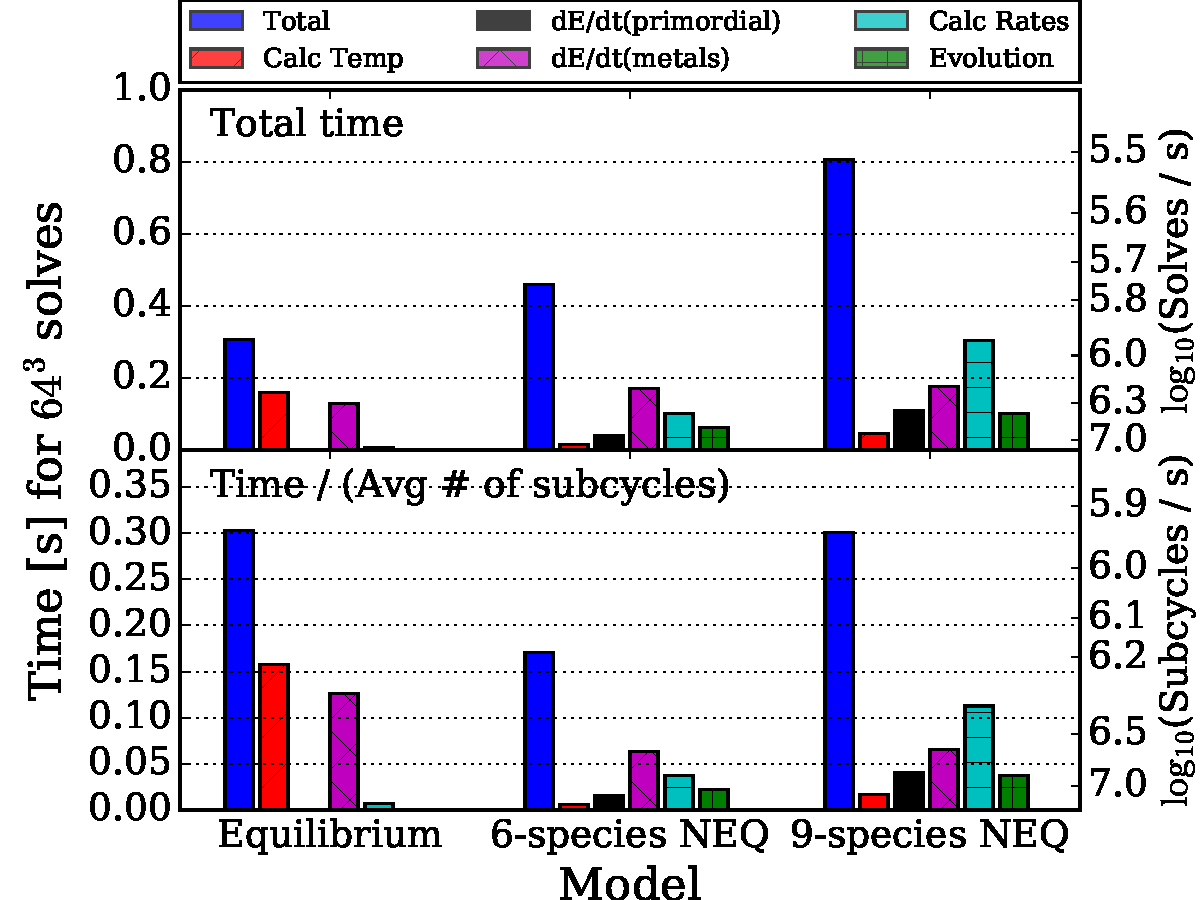
\includegraphics[width=0.98\textwidth]{figures/performance.pdf}
  \caption{Serial performance - Top: integration time for a 64$^{3}$
    element fluid container, with tabulated cooling (``equilibrium'',
    left), atomic chemistry (``6-species'', middle), and H$_{2}$ molecular chemistry
    (``9-species'', right).  Bottom: time normalized by the
    average subcycles per cell.  Colors denote the full solve
    (blue), temperature calculation (red), primordial (black) and metal
    (magenta) cooling calculation, and interpolation of rate
    coefficients (cyan).}
  \label{fig:single-proc}
\end{subfigure}%
\hspace{0.02\textwidth}
\begin{subfigure}{.42\textwidth}
  \centering
  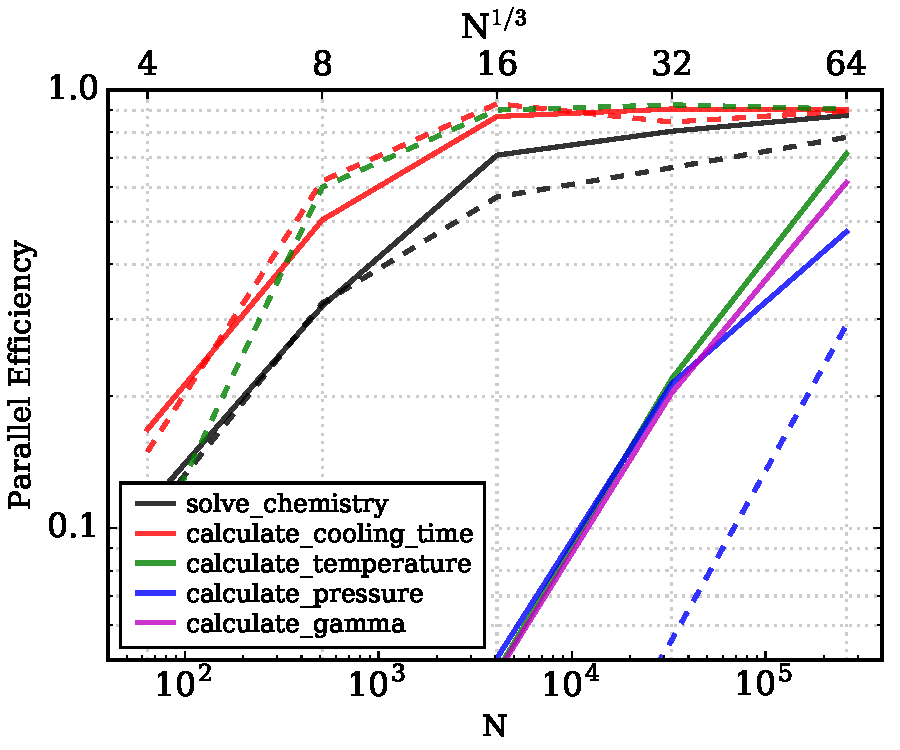
\includegraphics[width=0.98\textwidth]{figures/openmp.pdf}
  \caption{OpenMP parallel efficiency vs. size of fluid container for
    20 threads.  Solid lines show the molecular
    chemistry solver and dashed lines show the tabulated, equilibrium
    model.  For all expensive routines, the efficiency reaches
    $\sim$60\% to 90\% for $16^3$ cells and $\sim$80\% to 90\% for
    $64^3$ cells.}
  \label{fig:openmp}
\end{subfigure}%
\vspace*{-0.5\baselineskip}
\caption{Serial performance (left) and OpenMP efficiency of
  \grackle{'s} solvers \citep[from][]{2017MNRAS.466.2217S}.}
\label{fig:performance}
\vspace*{-0.5\baselineskip}
\end{figure}

In addition to the primordial chemistry and cooling, the contribution
to the total cooling rate by metals is calculated by linearly
interpolating over pre-computed tables of heating and cooling rates,
following the method of \citet{2008MNRAS.385.1443S}.
The metal cooling component is calculated within the same subcycle
iteration as the chemistry solver and contributes to the cooling time
time-step limiter.
If using a UV background model,
additional tables also provide photo-ionization, -dissociation, and
-heating rates for the various species.
The tables distributed with the source code are calculated with the
photo-ionization code, \texttt{Cloudy}, but can in principle be
generated by other similar codes, such as \texttt{Mappings III}
\citep{1993ApJS...88..253S}.

\noindent
{\bf Implementation}
All user-facing \grackle{} functions are written in C due
to the relative simplicity of calling C routines from other
languages, particularly C++ and Fortran.  Most of \grackle{}'s
internal functionality is written in Fortran to make use of the
language's efficient loop and array operations.
The internal machinery is optimized to work with a set of arrays of
densities and internal energies, referred to as a ``fluid
container'', where the arrays represent either a three-dimensional
grid with inactive ghost zones or a one-dimension set of particles.
The solvers are designed to make the best possible use of cache by
operating on field data in the order in which it is stored in memory.
The core computations are performed on
contiguous sub-segments of the field arrays to allow for loops to be
unrolled by compilers for more efficient vector operations.
%% For three-dimensional grids, these sub-segments are pencil-beams of all $i$
%% values for given values $k$ and $j$ in an $i\times j\times k$ cube.
%% For 1D arrays of particles, analogous divisions can be used to break
%% the arrays into multiple sub-segments to be passed to the core
%% functions.

\noindent
{\bf Performance}
In Figure \ref{fig:single-proc}, we
display performance results for \grackle{}'s different solvers.  For
this test, we initialize a 3D fluid container with 64$^{3}$ elements
with density, temperature, and metallicity varying smoothly in each
dimension and evolve it for a period of 500 years.  On the test
machine, \grackle{} performs
roughly 0.5-1$\times10^{6}$ full solves per second and at least
10$^{6}$ subcycles per second, depending only slightly on the choice
of solver.  Due to a lack of similar packages, an absolute evaluation
of this performance is difficult.  However, a comparison can be made
to the \texttt{Enzo} simulation code as a whole.
\citet{2014ApJS..211...19B} perform a weak scaling test of
\texttt{Enzo} with a simulation including gravity,
hydrodynamics, and a chemistry solver analogous to \grackle{}'s atomic
solver.  They find that \texttt{Enzo} optimally reaches about 10$^{5}$
full cell updates per second, suggesting that \grackle{} would consume
approximately 20-25\% of the computational cost.

\noindent
{\bf Parallelism}
Because \grackle{}'s functionality requires no communication and is
fully thread-safe once initialized, the library can be easily used
within a simulation code parallelized with a message passing framework
like MPI.  Additionally, all of \grackle{}'s functions are
parallelized with OpenMP by threading the outer loops over which the
solvers are called to operate on the field array sub-segments.  This
allows the library to work within hybrid MPI/OpenMP frameworks, such
as that adopted by the latest version of \texttt{Gadget}.
In Figure \ref{fig:openmp}, we show the OpenMP efficiency of
\grackle{}'s functions for the most and least complex versions
of the solver.  Here, we define parallel efficiency as the ratio of
multi- to single-thread performance.  The test is run using 20 OpenMP
threads for fluid container sizes from 4$^{3}$ to
64$^{3}$.  At 16$^{3}$ elements, the efficiency is 60-90\%
for all computationally expensive routines.  The four routines that
show relatively poor efficiency are very inexpensive and so contribute negligibly to
the total cost.
%% This parallelism can also help pure-MPI codes
%% where memory requirements force the use of fewer than the total number
%% of cores on a node.

\subsection{Community and Usage Metrics}

The first stable version of the \grackle{} library was released in
January 2014, with the most recent release (\grackle{} 3.1) on April
3, 2018.  Since the initial release, the \grackle{} API has been
implemented in 14 simulation codes and has been used in at least 48 papers
published in the Astrophysical Journal, Monthly Notices of the Royal
Astronomical Society, and Nature.  The paper topics include galaxy,
star, and black hole formation; dwarf
and disk galaxies; high redshift interstellar medium; Lyman-alpha
forest; history of the Milky Way; reionization; supernova
remnants; metal mixing; and turbulence.  Usage has grown steadily
from year to year, with 1 publication using \grackle{} in 2014, 5 in
2015, 11 in 2016, 22 in 2017, and 9 as of April, 2018.  The
\grackle{} mailing list currently has 76 subscribers, increasing by
roughly 15-20 per year.

Much of \grackle{}'s primordial chemistry solver was first developed
by Peter Anninos and collaborators in the mid-1990s
\citep{1997NewA....2..209A, 1997NewA....2..181A} and incorporated into
the simulation code, \texttt{Enzo} \citep[][licensed under the
  3-clause, revised BSD license]{2014ApJS..211...19B} a few
years later.  As a component of \texttt{Enzo}, the chemistry solver
was developed through contributions made by many in the
\texttt{Enzo} community, including PIs Britton Smith and Matthew Turk
and collaborators Greg Bryan and Simon Glover.  In response to a call for
a ``common physics package'' to enable a large, multi-simulation
comparison project \citep[AGORA,][]{2014ApJS..210...14K,
  2016ApJ...833..202K}, PI Smith extracted the chemistry and
cooling machinery from \texttt{Enzo} and converted it into a
stand-alone, linkable library with a number of improvements
and new features.  The first commit made to the \grackle{}
project was in October 2012.  Since then, the project has progressed
under the same philosophy of feature-driven, community development as
it had as a component of \texttt{Enzo}.  In that time, the code has
received commits from 16 different contributors and has had several different
``release managers" drawn from the community.

\subsection{Future Challenges}

The strength of the \grackle{} community is a testament to the
project's ability to meet the \textit{current} needs of its users.  However,
those needs will continue to evolve as the scientific frontier
advances and simulations increase in sophistication.  In order to
prioritize future development, a survey of \grackle{} users was
conducted in Spring 2017, allowing respondents to submit feature
requests.  Many of the highly desired features were newly published
models and minor enhancements, their implementation constituting
well-define development projects suitable for students.  Two of these
are included in the proposed work.  However, the most desired
capability (over 75\% of respondents) was the inclusion of additional
elements in the chemistry solver.  In addition to aiding current
users, this functionality would also open \grackle{} up to simulators
of present-day star formation and the local interstellar medium (ISM)
who require, minimally, the addition of C and O and their
associated molecules to \grackle{'s} current network.  Looking beyond
this, the ability to add even more complexity, including species of
N, F, and S as well as molecular isotopologues
\citep{2008ApJ...679..481P}, deuterated molecules
\citep{2005ApJ...619..379C}, polycyclic aromatic hydrocarbons
\citep[PAHs,][]{2016JPhCS.728f2005G}, and
additional dust variations \citep{2013RvMP...85.1021T}, will be crucial
to interpreting new observations coming from facilities like the
Atacama Large Millimeter/submillimeter Array (ALMA).
Yet, as the complexity and connectivity of the network increases, so
will the difficulty of implementation and the rate of error.  Keeping
pace with demands through manual development will become
untenable.  Instead, we propose a different strategy where complex
networks are machine-generated.

%% This SSE will establish \grackle{} as a vital software element for the
%% computational astrophysics community.  It will allow the code to adapt
%% to the latest technologies that will enable the next generation of
%% simulations.  It will expand the capabilities of \grackle{} to reach a
%% larger audience and provide a venue for collaboration and
%% dissemination of new research.
